\section{Grundlagen}

	\subsection{Eingabegeräte für Schwerstmehrfachbehinderte}
    \label{sec:input-devices}
    
    	Aufgrund der Vielzahl an möglichen Behinderungen und Einschränkungen gibt es eine mindestens genau so große Zahl an Eingabemethoden und Geräten. Diese Eingabegeräte können sowohl eine Schnitstelle zu klassischen PCs darstellen oder auch zur Bedienung von unterstützenden Technologien wie z. B. eines Rollstuhls benutzt werden. Im Folgenden sollen hier exemplarisch einige solcher Eingabegeräte vorgestellt werden. Die hier vorgestellte Auswahl ist nicht vollständig und ist aus den Onlinekatalogen der \emph{RehaMedia GmbH}, und der \emph{REHAVISTA GmbH} sowie den Webseiten der erwähnten Hersteller zusammengetragen.
        
        \subsubsection*{Augensteuerung}
        	Bei der Augensteuerung werden mit Hilfe einer Kamera die Bewegungen der Augen genutzt um ein Gerät zu steuern. Damit können dann auch Windows oder OS X Betriebssysteme mit Hilfe eines On-Screen-Menüs gesteuert werden. Der Anbieter \emph{RehaMedia} bewirbt das System \emph{Tobii PCEye} mit den Worten: \enquote{Die Augensteuerung erfasst die Augenbewegungen und setzt sie präzise in Mausbewegungen um. Dank eines Mauszeigermenüs stehen auch bei der Bedienung mit der Augensteuerung alle Mausfunktionen wie Doppelklick, Rechtsklick usw. zur Verfügung.} \parencite{rehamedia:TobiiPCEyeGo}
            
         \subsubsection*{Taster}
         	In der Regel handelt es sich bei Tastern um einen einzelnen großen runden Knopf (\autoref{fig:bigRed}). Es gibt aber auch andere Ausführungen wie einen Griff, welchen man zusammendrücken kann oder einen befestigten Stab gegen den man Druck ausüben kann. Manche Taster können auch an der Kleidung oder an einer Kopfstütze angebracht werden, so dass eine Bedienung nicht nur mit den Händen sondern auch mit dem Kopf oder durch zusammenschlagen der Knie möglich ist. Pedale zur Bedienung mit den Füßen werden auch angeboten. Die meisten Taster verwenden einen 3,5 mm Klinkenstecker und können damit ein diskretes Signal senden. Der Hersteller \emph{ablenet} bietet z. B. Spielsachen an, die so gesteuert werden können (\autoref{fig:penguinRace}). Andere Eingabegeräte können auch Anschlüsse für diese Taster bereitstellen so das diese kombiniert werden können.  
         	
            \begin{figure}[H]
				\centering
				\begin{subfigure}{.49\textwidth}
  					\centering
  					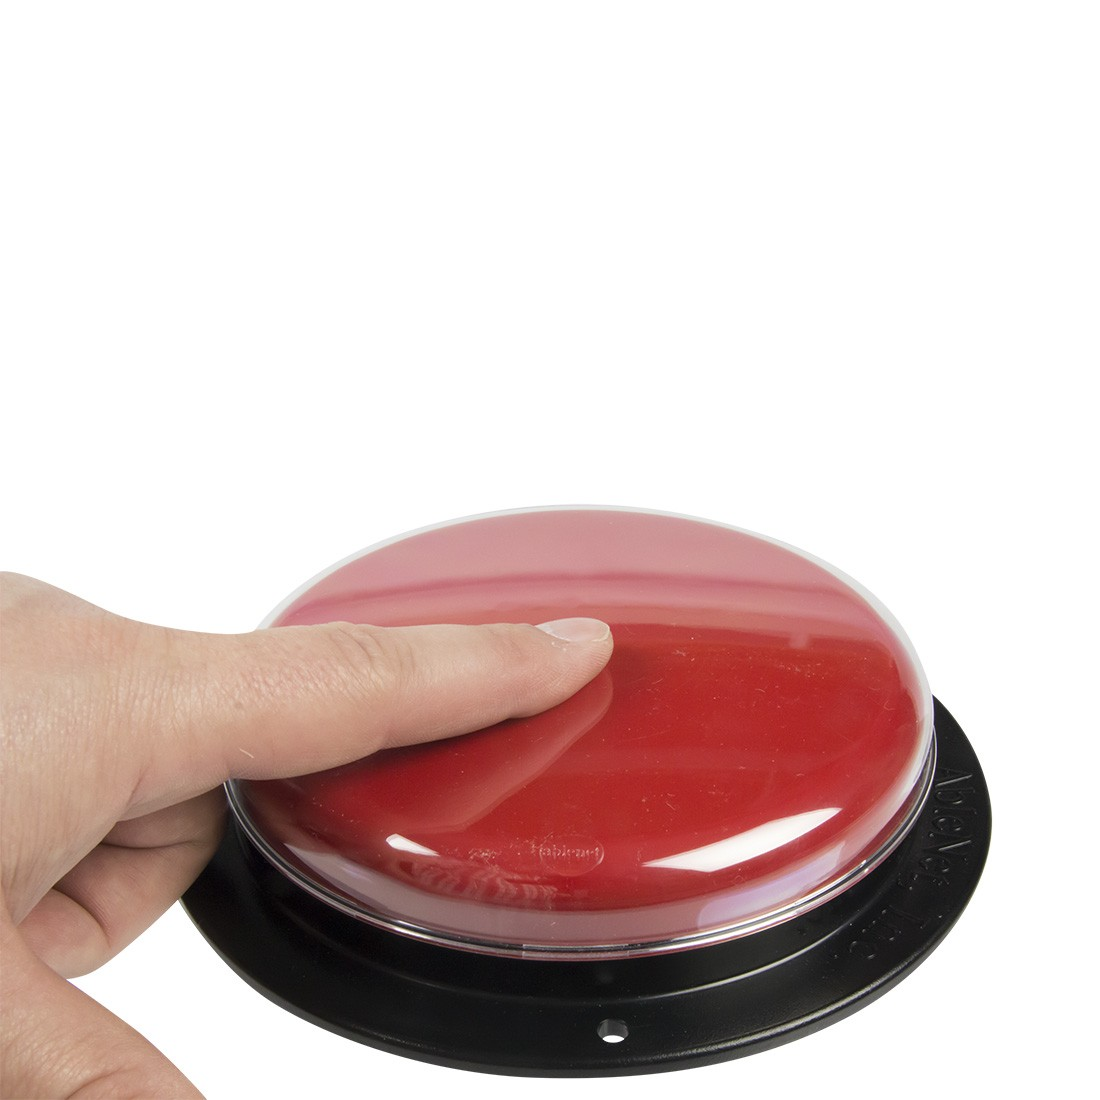
\includegraphics[width=.8\linewidth]{images/big-red-button.jpg}
  					\caption{\emph{Big Red} \cite{ablenet:bigRed}}
                    
  					\label{fig:bigRed}
				\end{subfigure}
				\begin{subfigure}{.49\textwidth}
  					\centering
  					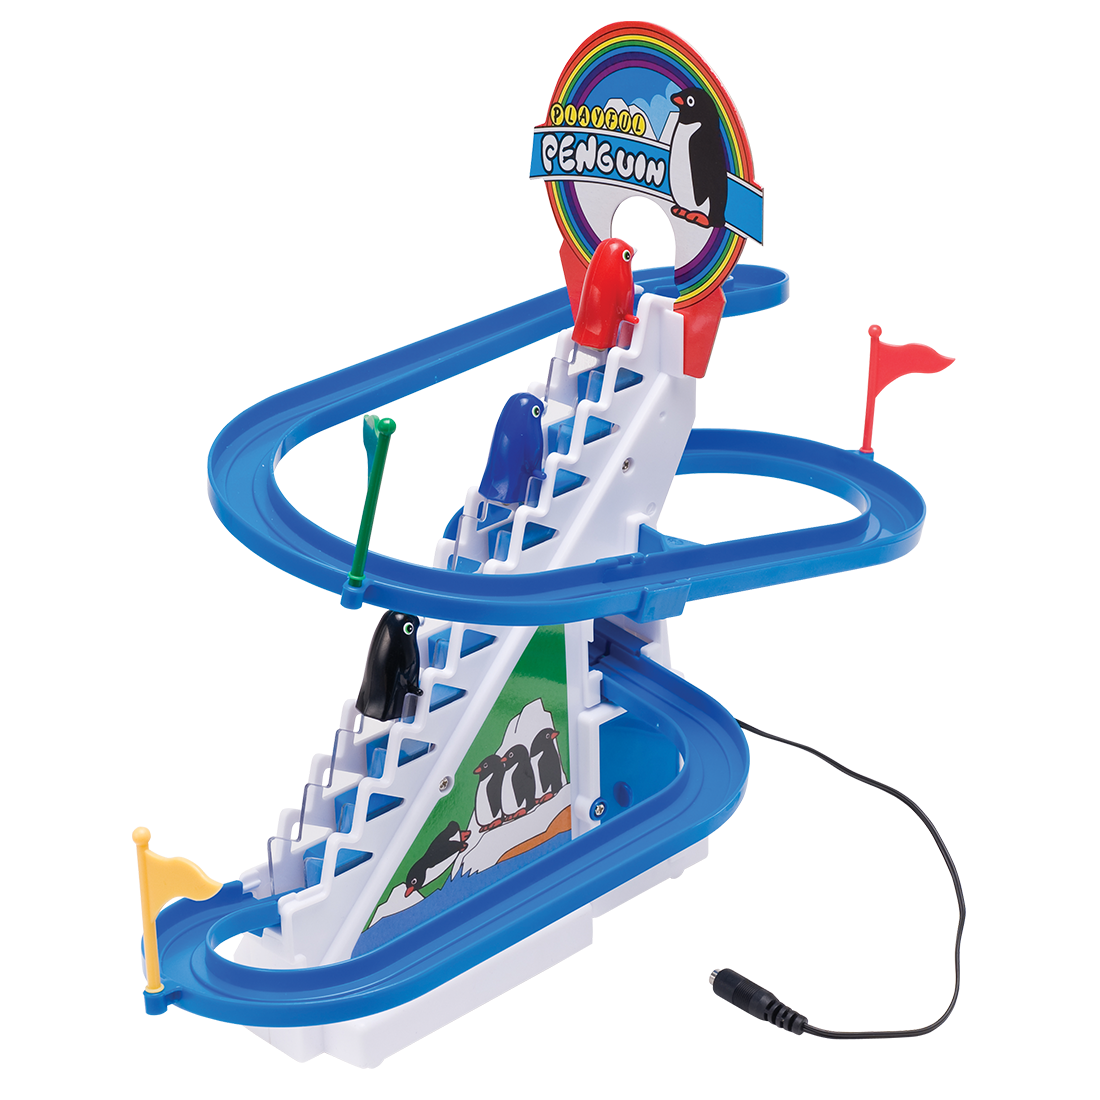
\includegraphics[width=.8\linewidth]{images/penguin-race.png}
  					\caption{\emph{Penguin Race} \cite{ablenet:penguinRace}}
  					\label{fig:penguinRace}
				\end{subfigure}
                \caption{Taster und Spielzeug von ablenet}
				\label{fig:ablenetSingleButtons}
			\end{figure}
            
            Eine weitere Ausführung sind \emph{sprechende Tasten}. Diese Taster haben einen Lautsprecher eingebaut und bieten die Möglichkeit eine oder mehrere Sprachnachrichten aufzunehmen. Wenn mehrere Nachrichten aufgenommen werden können, kann die auszugebende Nachricht von einer betreuenden Person voreingestellt werden. Andere Geräte funktionieren nach dem Prinzip: einmal drücken gibt Nachricht Nummer eins aus, zweimal drücken Nachricht Nummer zwei und dreimal drücken Nachricht Nummer drei.
            
        	Außerdem gibt es Taster mit mehr als einer Taste. Diese sind dann schon zum Anschluss an Computer oder Tablets gedacht und haben häufig einen \emph{USB} oder \emph{Bluetooth} Anschluss. Der Tastenumfang geht dabei von einfachen Geräten mit zwei Tasten bis zu kompletten Computertastaturen.
            
            \begin{figure}[H]
				\centering
				\begin{subfigure}{.33\textwidth}
  					\centering
  					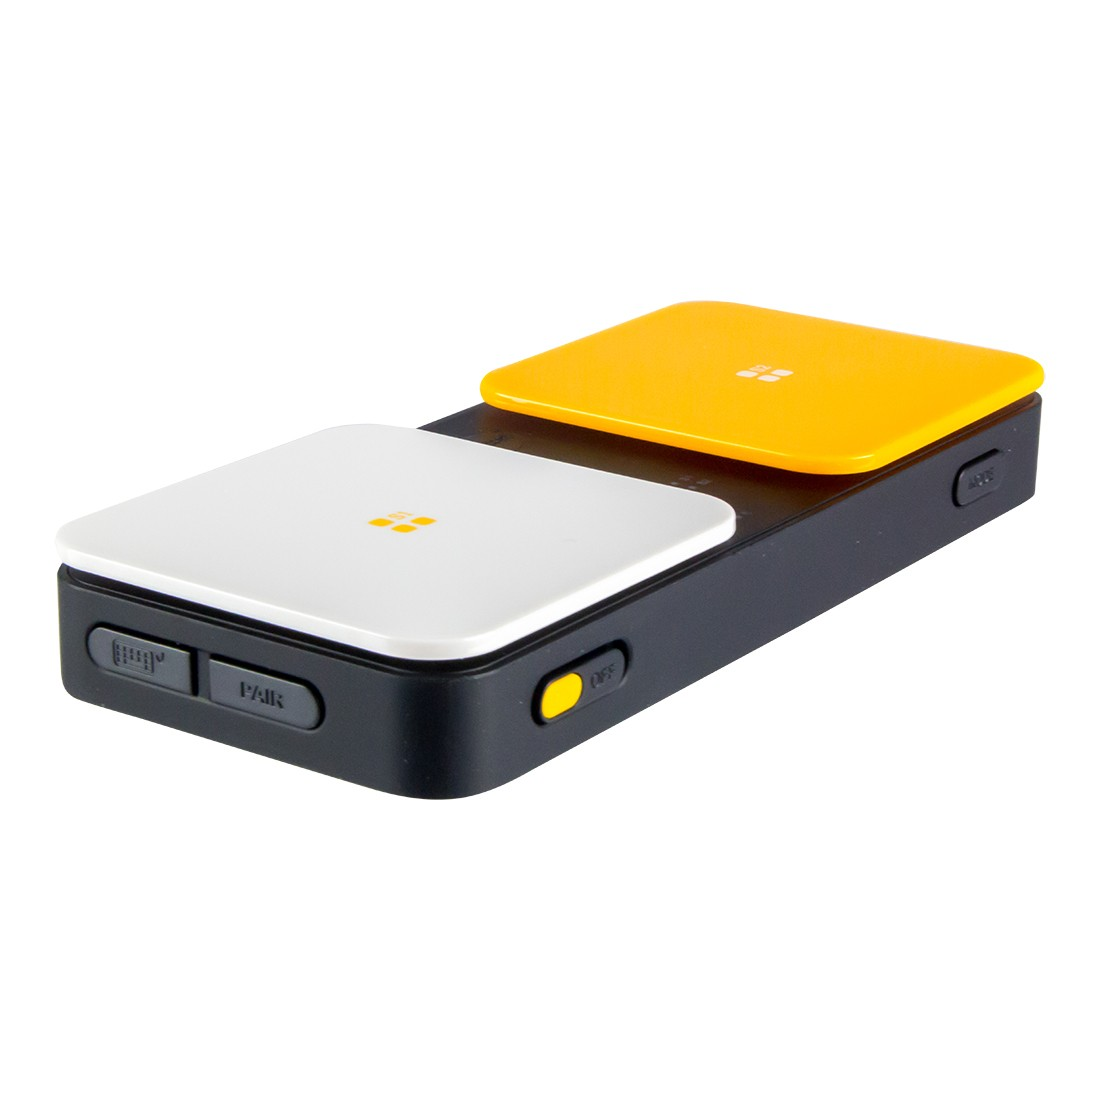
\includegraphics[width=.8\linewidth]{images/buttonsIPad.jpg}
  					\caption{\cite{ablenet:iPad}}
                    
				\end{subfigure}%
				\begin{subfigure}{.33\textwidth}
  					\centering
  					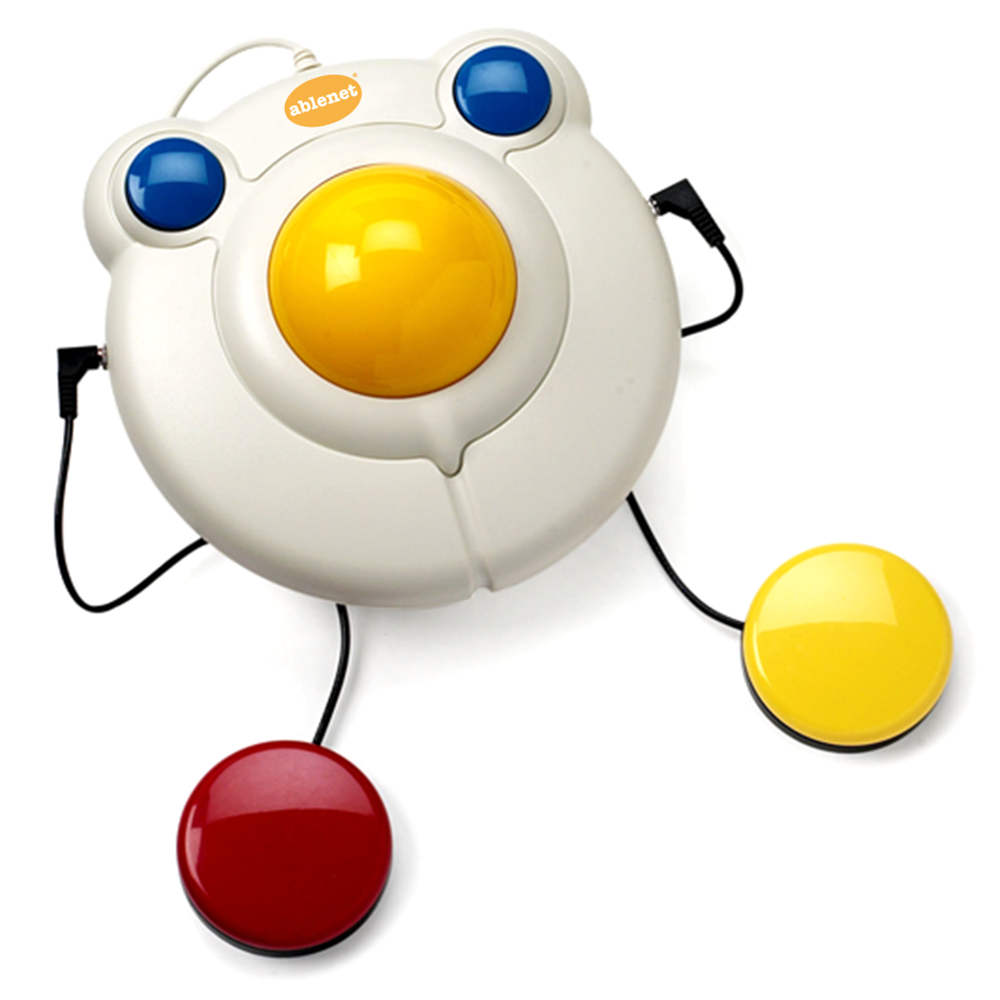
\includegraphics[width=.8\linewidth]{images/buttonsMouse.png}
  					\caption{\cite{ablenet:mouse}}
				\end{subfigure}
                \begin{subfigure}{.33\textwidth}
  					\centering
  					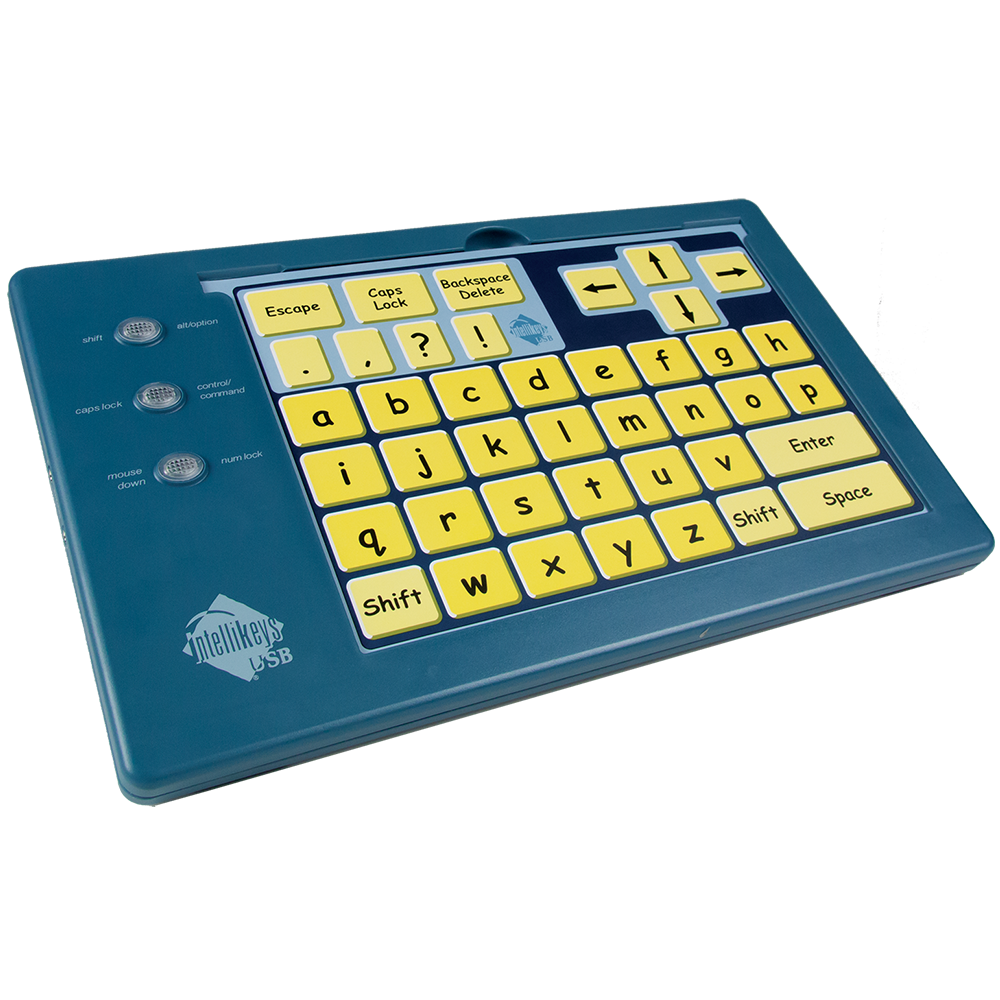
\includegraphics[width=.8\linewidth]{images/buttonsKeyboard.png}
  					\caption{\cite{ablenet:keyboard}}
				\end{subfigure}
                \caption{Taster mit mehreren Tasten von ablenet}
				\label{fig:ablenetMultipleButtons}
			\end{figure}
            
		\subsubsection*{Talker}
        	Bei Talkern handelt es sich um Geräte mit denen durch Knopfdruck Sprache ausgegeben werden kann. Es existieren sowohl statische als auch dynamische Systeme. Bei statischen Systemen sind die Knöpfe fest in der Hardware eingebaut. Dynamische Systeme verwenden Touchscreens. Oft werden dafür auch handelsübliche Tablets mit Schutzhüllen und Halterungen verwendet. 
            
            Diese Systeme können unterschiedlich komplex sein. Einfachere Talker haben ein festes Set an Symbolen, welche auf Knopfdruck Sprachnachrichten ausgeben. Dynamische Systeme ermöglichen die Navigation durch verschiedene Symbolgruppen oder arbeiten sogar nur mit Text. Manche ermöglichen auch eine Texteingabe per Tastatur. In \autoref{sec:software-examples} werden verschiedene Softwarelösungen für solche Systeme vorgestellt.
            
            \begin{figure}[H]
				\centering
				\begin{subfigure}{.3\textwidth}
  					\centering
  					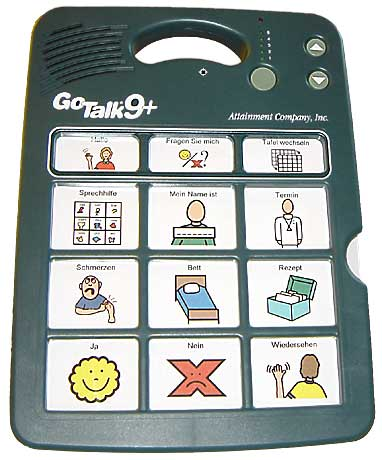
\includegraphics[width=.8\linewidth]{images/goTalkPlus.jpg}
  					\caption{statischer Talker \parencite{rehavista:goTalkPlus}}
                    
				\end{subfigure}
				\begin{subfigure}{.3\textwidth}
  					\centering
  					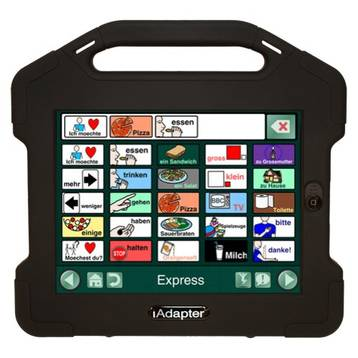
\includegraphics[width=.8\linewidth]{images/goTalkNow.jpg}
  					\caption{iPad mit Talker Erweiterung \parencite{rehamedia:goTalkNow}}
				\end{subfigure}
                \begin{subfigure}{.3\textwidth}
  					\centering
  					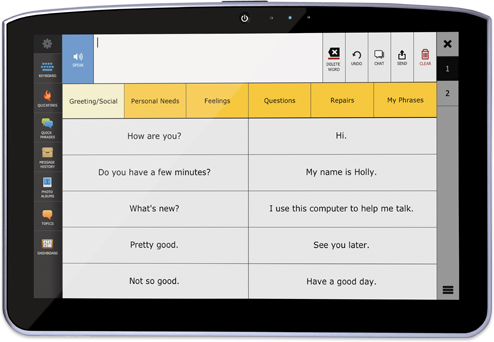
\includegraphics[width=.8\linewidth]{images/tobiiT15.png}
  					\caption{Talker mit literarischem Interface \parencite{tobii:T15}}
                    \label{fig:tobiiT15}
				\end{subfigure}
                \caption{verschiedene Talker}
				\label{fig:talker}
			\end{figure}
            
    \newpage
    
    \subsection{Software für Unterstützte Kommunikation}
    \label{sec:software-examples}
    
    	Unter Sprachsoftware wird hier das komplette System von Benutzeroberfläche über mögliche Autovervollständigungen und Eingabevorschlägen bis zur Sprachausgabe verstanden. Im speziellen soll hier Software vorgestellt werden, die auf den in \autoref{sec:input-devices} beschriebenen \emph{Talkern} Anwendung findet. Die Auswahl der Beispiele richtet sich an ihrer Rleveanz für den zu entwickelnden Prototypen. Software deren Funktion den in \autoref{sec:requirements} formulierten Anforderungen nahe kommt.
        
        \subsubsection*{MetaTalkDE / MetaTalkUS}
        	\emph{MetaTalkDE} ist eine iPad App von \emph{Cidar Health Care LLC} für Symbolbasierte \emph{Unterstützte Kommunikation}.
            
            \begin{figure}[H]
				\centering
				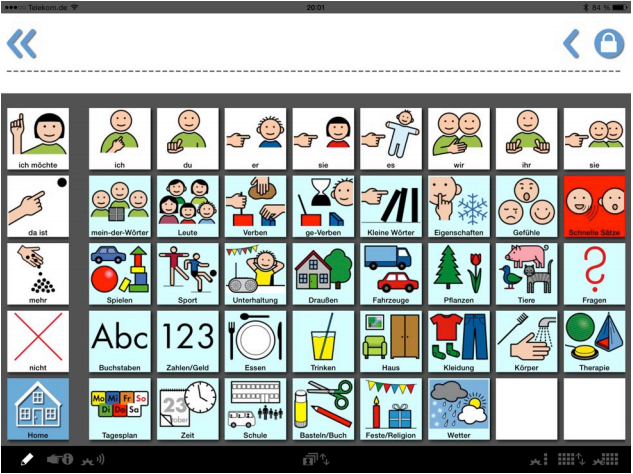
\includegraphics[width=.65\linewidth]{images/Metatalk.png}
                \caption{Schreenshot von MetaTalkDE in der 5x9 Ansicht
                	\parencite[S. 8]{cidar:metaTalkManual}
                }
				\label{fig:metatalk}
			\end{figure}
            
            Auf dem Startbildschirm werden oben in einer Zeile vom Nutzer bereits Ausgewählte Symbole angezeigt. Darunter befindet sich ein Raster mit Symbolen und Kategorien. Durch Auswahl einer Kategorie gelangt man auf einen neuen Bildschirm mit entsprechenden Symbolen.
            Durch Druck auf die Symbolzeile oben werden die gelisteten Symbole gesprochen. 
            Laut Handbuch \parencite[S. 7 ff]{cidar:metaTalkManual} ist die Anzahl der Tasten im Raster ist in drei Stufen (5x9, 4x7, 3x5) anpassbar. Beim Anpassen des Rasters wird auch das Vokabular angepasst. Jede Stufe hat auch ein eigenes Vokabular, wobei standartmäßig mehr Tasten auch ein größeres Vokabular bedeuten. Die Vokabulare sind innerhalb der App editierbar und können wie auf Seite 20 f erklärt auch über E-Mail ex- und importiert werden. Die gesamte App bietet viele Möglichkeiten der Personalisierung. So können die Symbole der Tasten ausgetauscht werden, neue Tasten hinzugefügt werden, Tasten mit Farben hinterlegt werden und auch Töne für die Sprachausgabe aufgenommen werden (vgl. S.24). Nach Auswahl von Personalpronomen werden die Verben in der passenden Form angezeigt. Dazu lassen sich durch langes Drücken auf ein Symbol andere Formen des entsprechenden Wortes anzeigen. (vgl. S.11 – 14) Auch wird auf Seite 33 erleutert wie sich \emph{Verlinkungen} erstellen lassen, mit denen darauffolgende Symbollisten angezeigt werden.
            
            Da die App auf einem iPad läuft, muss der Nutzer motorisch in der Lage sein diese mit den Händen zu bedienen. Zwar gibt es die oben beschriebenen \emph{Verlinkungen}, jedoch nutzt die App keine Methoden des \emph{Mashine learning}, um die Eingabe durch optimierte Symbollisten zu erleichtern.
            
        \subsubsection*{Tobii Sono Scribe}
        
        	\emph{Tobii Sono Scribe} ist eine Erweiterung zu der Software \emph{Tobii Communicator}. Die Eingbe ist Textbasiert. Das Handbuch \parencite[S. 8]{tobii:sonoScribeManual} beschreibt zwei verschiedene Modi. In einem Modus wird mit einer Liste von vorgeschlagenen Wörtern gearbeitet (\autoref{fig:sonoScribeWords}), in dem anderen wird eine Displaytastatur zur Texteingabe verwendet (\autoref{fig:sonoScribeKeyboard}).
            
            \begin{figure}[H]
				\centering
				\begin{subfigure}{.49\linewidth}
  					\centering
  					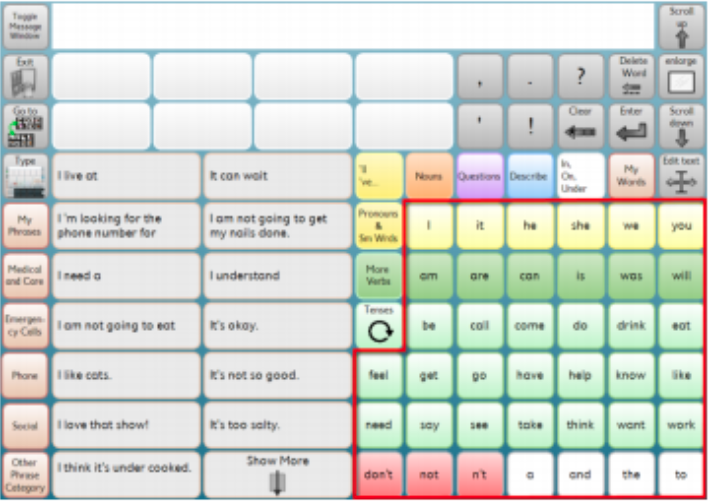
\includegraphics[width=.8\linewidth]{images/sonoScribeWords.png}
  					\caption{Wort Modus 
                    	\parencite[S. 13]{tobii:sonoScribeManual}
                    }
                    \label{fig:sonoScribeWords}
				\end{subfigure}
				\begin{subfigure}{.49\linewidth}
  					\centering
  					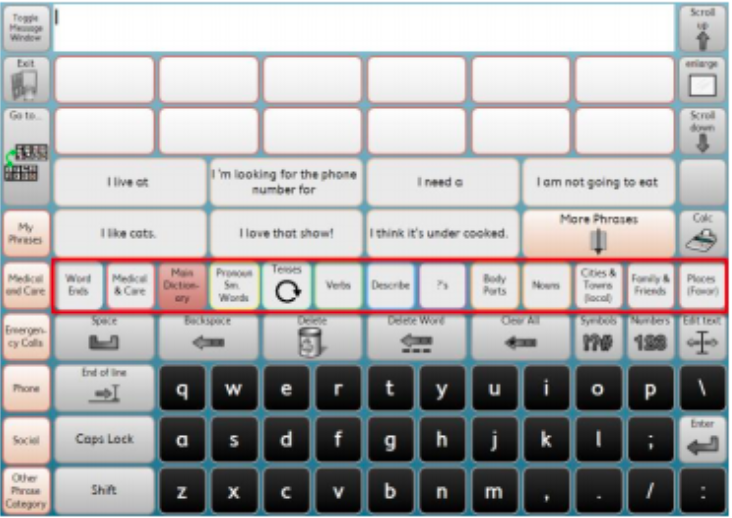
\includegraphics[width=.8\linewidth]{images/SonoScribeKeboard.png}
  					\caption{Tastatur Modus 
                    	\parencite[S. 22]{tobii:sonoScribeManual}
                    }
                    \label{fig:sonoScribeKeyboard}
				\end{subfigure}
                \caption{ }
                \label{fig:sonoScribe}
			\end{figure}
        	
            Die Software kann unter Windows und auf den Geräten von \emph{Tobii}installiert werden. Zum Beispiel auf dem in \autoref{fig:tobiiT15} gezeigtem \emph{T15}. Neben dem Enthaltenen Vokabular werden auch verschiedene Listen mit häufig verwendeten Sätzen angeboten wie, auf S. 15 f des Handbuchs beschrieben wird. Sowohl das die Sätze und wie auf S. 20 ergänzt wird, das Vokabular sind innerhalb der Software editierbar.
            
            Bei der Eingabe werden wie auf S. 15 beschrieben mögliche nächste Wörter vorgeschlagen und auch Sätze mit entsprechenden Anfängen aus den gespeicherten Sätzen vorgeschlagen. Im tastaturbasierten Modus werden auch Wortvervollständigungen angeboten (Siehe S. 22). Auf S. 18 wird erklärt, dass Nutzer sich, wie in \autoref{fig:sonoScribeList} zu sehen, auch Listen von Wörtern sortiert nach der Wortart anzeigen lassen können.
            
            \begin{figure}[H]
  				\centering
  				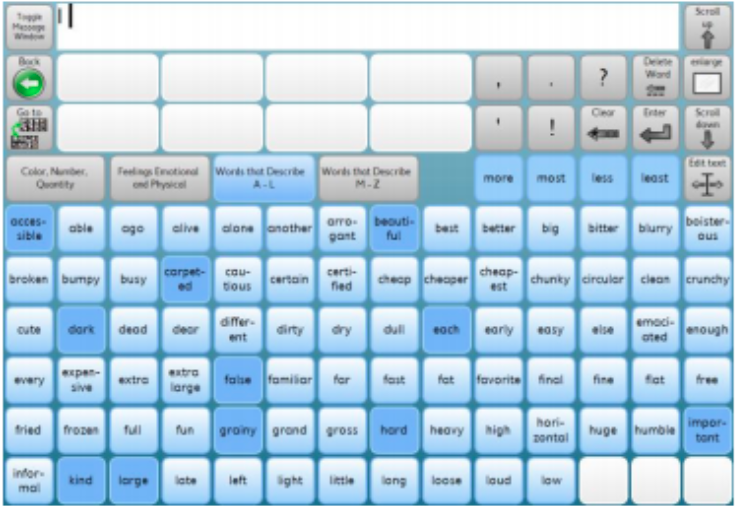
\includegraphics[width=.5\linewidth]{images/SonoScribeList.png}
  				\caption{Liste von Nomen \parencite[S. 18]{tobii:sonoScribeManual}}
                \label{fig:sonoScribeList}
			\end{figure}
            
			Neben der Sprachausgabe gibt es auch einen Texteditor, einen Mailclienten sowie verschiedne Tools zur Steureung des Windows Betriebssystems. Dazu gehört auch ein PlugIn für den Browser \emph{Mozilla Firefox}. Diese große Anzahl an Funktionionen setzt aber vorraus, dass Nutzer lesen und schreiben können müssen und fähig sind die im Vergleich mit \emph{MetaTalkDE} komplexe Benutzeroberfläche bedienen können. Die Software unsterstützt unter anderem die Eingabe per Touch, Augensteuerung und sogar durch Taster. Bei der Bedienung mit Taster gibt es ein \emph{Scan Raster} nach dem per Tastendruck von Knopf zu Knopf gesprungen wird.
    
	\subsection{Mashine learning Software in für den Massenmarkt}
    \emph{Mashine learning} zur Wortvorhersage wird nicht nur in der \emph{Unterstützten Kommunikation} angewendet sondern auch in Software für den Massenmarkt. Im folgenden sollen hier kurz drei Beispile vorgestellt werden, die Nutzern Worte zur Eingabe vorschlagen.
        
        \subsubsection*{swiftKey}
        	In einem Artikel für die Webseite \emph{techrepublic.com} beschreibt \cite{techrepublic:swiftKey} die Funktionen der Bildschirmtastatur für Mobile Geräte \emph{swiftKey}. Zuerst erwähnt er, wie Nutzern dank eines lernfähigen Algorythmus Worte vorgeschlagen werden. Im optimalen Fall müsste man also nach eingabe des ersten Wortes gar nicht mehr tippen. Dann beschreibt er die zweite Funktion welche \emph{Flow} genannt wird. Hierbei wird zum Tippen nicht abgesetzt, sondern mit dem Finger von einem Buchstaben zum anderen gewischt. Die Tastatur kann auch so das gewünschte Wort erkennen.
        
        \subsubsection*{iOS QuickType}
        
        	Die Bildschirmtastatur für \emph{Apple iOS 8} enthält ein Feature mit dem Namen \emph{QuickType}. Die Funktion ist ähnlich zu \emph{swiftKey} auch hier werden beim tippen Worte vorgeschlagen. \emph{Apple} bewirbt auf seiner Webseite, dass die Wortvorschläge Kontextabhängig sind. So wird beschrieben, dass in einem Mailprogramm andere Worte vorgeschlagen werden als in einem Chat mit einem Freund. Außerdem kann die Tastatur laut \cite{apple:quickType} auch eingehenden Text in einer Chatapplikation analysieren und entsprechende Vorschläge für die Antwort machen. Eine Funktion zum tippen ohne abzusetzen gibt es nicht.
        
        \subsubsection*{Google Suggest}
        
        	Auch \emph{Google} schlägt Nutzern Worte vor, während diese Begriffe in die Suchmaschine eingeben. Dieser Service nennt sich \emph{Google Suggest}. Dies beschreibt \cite{google:suggestIntro} im offiliellen Blog von Google. Außerdem erwähnt sie, dass der Service auch Rechtschreibfehler verbessern kann. In einem anderen Blogeintrag erklärt \cite{google:suggestUpdate} dass \emph{Goggle} 2\% der eingegeben Suchanfragen zusammen mit der IP-Adresse des Nutzers auswertet und aus diesen Daten die Vorschläge generiert.
    
    
    
    \newpage